\documentclass[tikz,border=10pt]{standalone}
\usepackage{tikz}
\usetikzlibrary{shapes.geometric, arrows, positioning, fit, backgrounds, shadows}

% --- Define Professional Styles ---
\tikzstyle{sensor} = [rectangle, rounded corners, minimum width=3cm, minimum height=1cm,text centered, draw=black, fill=red!10, drop shadow]
\tikzstyle{process} = [rectangle, minimum width=3cm, minimum height=1cm, text centered, draw=black, fill=orange!10, drop shadow]
\tikzstyle{model} = [rectangle, rounded corners, minimum width=4cm, minimum height=1.5cm, text centered, draw=black, fill=blue!10, drop shadow, line width=1.5pt]
\tikzstyle{output} = [rectangle, rounded corners, minimum width=3cm, minimum height=1cm, text centered, draw=black, fill=green!10, drop shadow]
\tikzstyle{arrow} = [thick,->,>=stealth]

\begin{document}

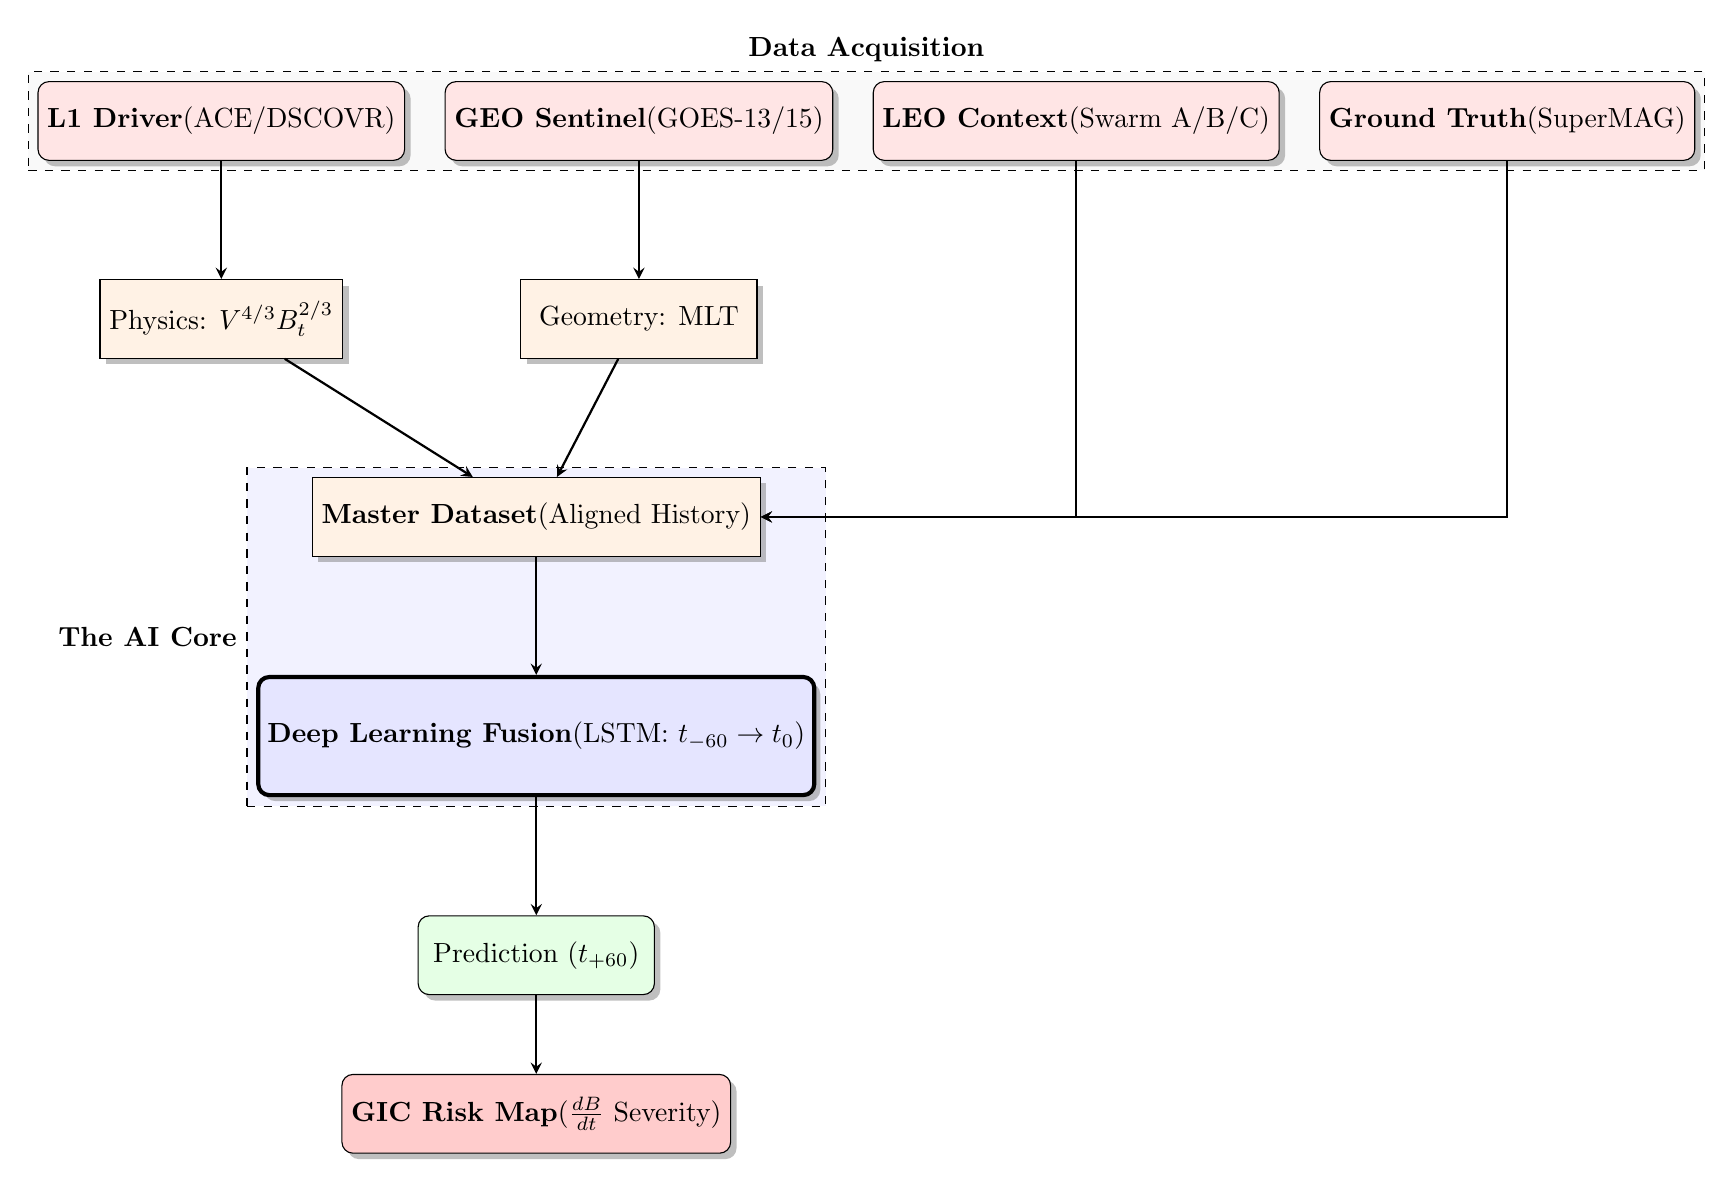
\begin{tikzpicture}[node distance=2cm]

% --- Phase 1: Inputs (Data Acquisition) ---
\node (L1) [sensor] {\textbf{L1 Driver} \\ (ACE/DSCOVR)};
\node (GOES) [sensor, right=0.5cm of L1] {\textbf{GEO Sentinel} \\ (GOES-13/15)};
\node (Swarm) [sensor, right=0.5cm of GOES] {\textbf{LEO Context} \\ (Swarm A/B/C)};
% --- THE MISSING PIECE ---
\node (Ground) [sensor, right=0.5cm of Swarm] {\textbf{Ground Truth} \\ (SuperMAG)};

% --- Phase 2: Feature Engineering ---
\node (Physics) [process, below=1.5cm of L1] {Physics: $V^{4/3} B_t^{2/3}$};
\node (Geom) [process, below=1.5cm of GOES] {Geometry: MLT};

% --- Phase 3: Fusion ---
\node (Master) [process, below=1.5cm of Physics, xshift=4cm] {\textbf{Master Dataset} \\ (Aligned History)};
\node (LSTM) [model, below=1.5cm of Master] {\textbf{Deep Learning Fusion} \\ (LSTM: $t_{-60} \to t_0$)};

% --- Phase 4: Output ---
\node (Prediction) [output, below=1.5cm of LSTM] {Prediction ($t_{+60}$)};
\node (Risk) [output, below=1cm of Prediction, fill=red!20] {\textbf{GIC Risk Map} \\ ($\frac{dB}{dt}$ Severity)};

% --- Arrows ---
\draw [arrow] (L1) -- (Physics);
\draw [arrow] (GOES) -- (Geom);
\draw [arrow] (Swarm) |- (Master);
\draw [arrow] (Ground) |- (Master); % Connect SuperMAG to Dataset
\draw [arrow] (Physics) -- (Master);
\draw [arrow] (Geom) -- (Master);
\draw [arrow] (Master) -- (LSTM);
\draw [arrow] (LSTM) -- (Prediction);
\draw [arrow] (Prediction) -- (Risk);

% --- Background Boxes ---
\begin{pgfonlayer}{background}
    \node [fit=(L1) (Ground), fill=gray!5, draw, dashed, label=above:\textbf{Data Acquisition}] {};
    \node [fit=(Master) (LSTM), fill=blue!5, draw, dashed, label=left:\textbf{The AI Core}] {};
\end{pgfonlayer}

\end{tikzpicture}

\end{document}